%!TEX root=main.tex
\section{Gilbert Runtime}
\label{sec:gilbertRuntime}

The Gilbert runtime is responsible for executing the compiled MATLAB code on a particular platform.
For this purpose, it receives the intermediate representation of the code and translates it into the execution engine's specific format.
Currently, Gilbert supports three different execution engines: \emph{ReferenceExecutor}, \emph{StratosphereExecutor} and \emph{SparkExecutor}.
The \emph{ReferenceExecutor} executes the compiled MATLAB code locally.
For the distributed execution Gilbert supports the Spark and the Stratosphere system as backends.

The \emph{ReferenceExecutor} is an interpreter for the intermediate code.
It takes the dependency tree of a MATLAB program and executes it by evaluating the operators bottom-up.
In order to evaluate an operator, the system first evaluates all inputs of an operator and then executes the actual operator logic.
Since the program is executed locally, the complete data of each operator is always accessible and, thus, no communication logic is required.
All input and output files are directly written to the local hard drive.

In contrast to the \emph{ReferenceExecutor}, the \emph{StratosphereExecutor} executes the program in parallel.
It takes the dependency tree of a MATLAB program and translates it into a PACT plan.
After the plan is generated, it is issued to the Stratosphere system for parallel execution.
This approach implies that the program is not directly executed by the executor.
Instead, the executor represents just another translation step.

The PACT plans are executed in parallel.
Consequently, data structures are needed which can be distributed across several nodes and represent the commonly used linear algebra abstractions, such as vectors and matrices.
Moreover, the linear algebra operations have to be adjusted so that they keep working in a distributed environment.
Fortunately, Stratosphere offers a rich and expressive API to easily realize distributed computations.
The details of the distributed data structures and operations are explained in \cref{sec:DistributedMatrixRepresentation} and \cref{sec:LinearAlgebraOperations}.

The \emph{SparkExecutor} is the second executor for distributed computations.
In contrast to the \emph{StratosphereExecutor}, it executes the MATLAB programs on top of the Spark system.
Since Spark and Stratosphere offer a similar set of programming primitives, they can both operate on the same data structures.
Furthermore, even most of the linear algebra operations can be implemented similarly.
The only programming difference is the incremental plan roll out feature of Spark.
By emitting Spark transformations and actions, the user can trigger computations in the cluster and retrieve intermediate results on the driver node.
This feature allows a more interactive way of programming, manifesting in a more natural way loops are defined, for example.
However, these differences are only subtle and do not limit or extend the expressiveness of either system.

\subsection{Distributed Matrix Representation}
\label{sec:DistributedMatrixRepresentation}

One aspect of writing distributed algorithms is how the relevant data is distributed across several worker nodes.
Since the distribution pattern directly influences the algorithms, one cannot consider them independently from one another.
In Gilbert's use case, the main data structure are matrices.
Thus, a partitioning for matrices has to be conceived which allows efficient algorithms working on the distributed data.
Looking at a matrix, one easily finds a multitude of different partition schemes.

A first idea could be to partition a matrix according to their rows or columns, as it is depicted in \cref{fig:rowPartitioning} and \cref{fig:columnPartitioning}.
This scheme allows to represent a matrix as a set of vectors which is stored in a distributed fashion.
Furthermore, it allows an efficient realization of cellwise operations, such as $+,-,/$ or $.*$.
In order to calculate the result of such an operation, we only have to join the corresponding rows of both operands and execute the operation locally for each pair of rows.

\begin{figure}
	\centering
	\begin{subfigure}{.3\linewidth}
		\centering
		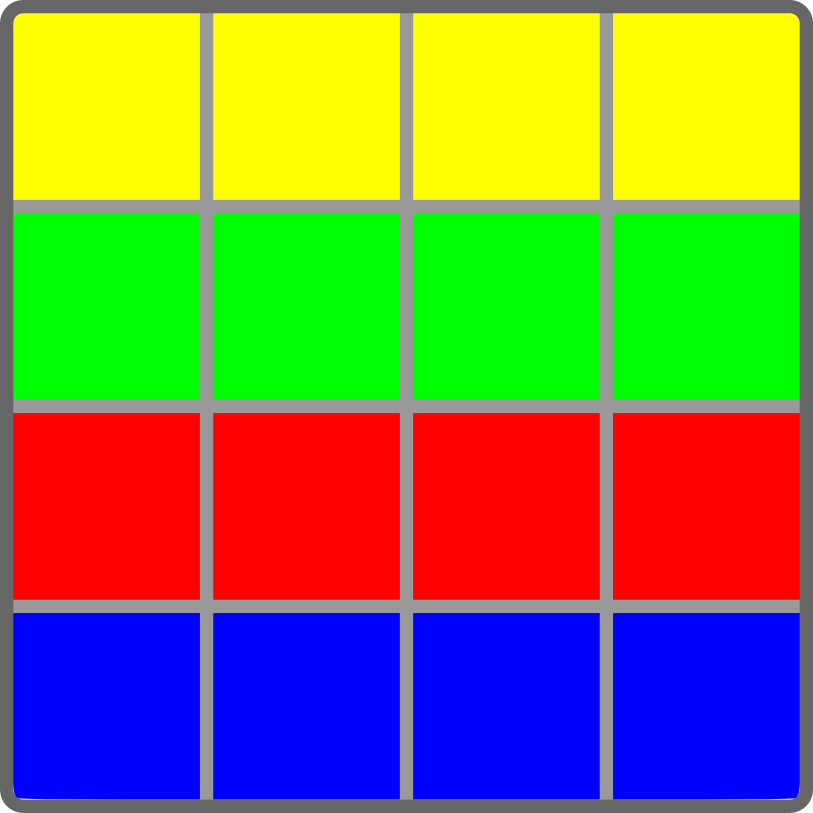
\includegraphics[width=0.55\textwidth]{images/rowPartitioning.png}
		\caption{Row partitioning}
		\label{fig:rowPartitioning}
	\end{subfigure}
	\begin{subfigure}{.3\linewidth}
		\centering
		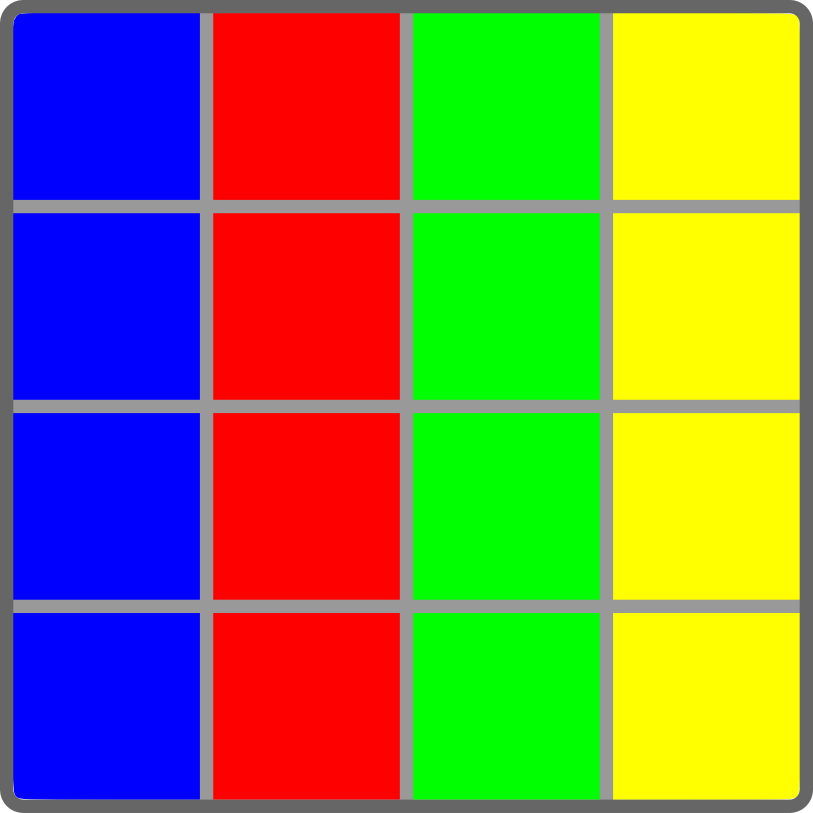
\includegraphics[width=0.55\textwidth]{images/columnPartitioning.png}
		\caption{Column partitioning}
		\label{fig:columnPartitioning}
	\end{subfigure}
	\begin{subfigure}{.3\linewidth}
		\centering
		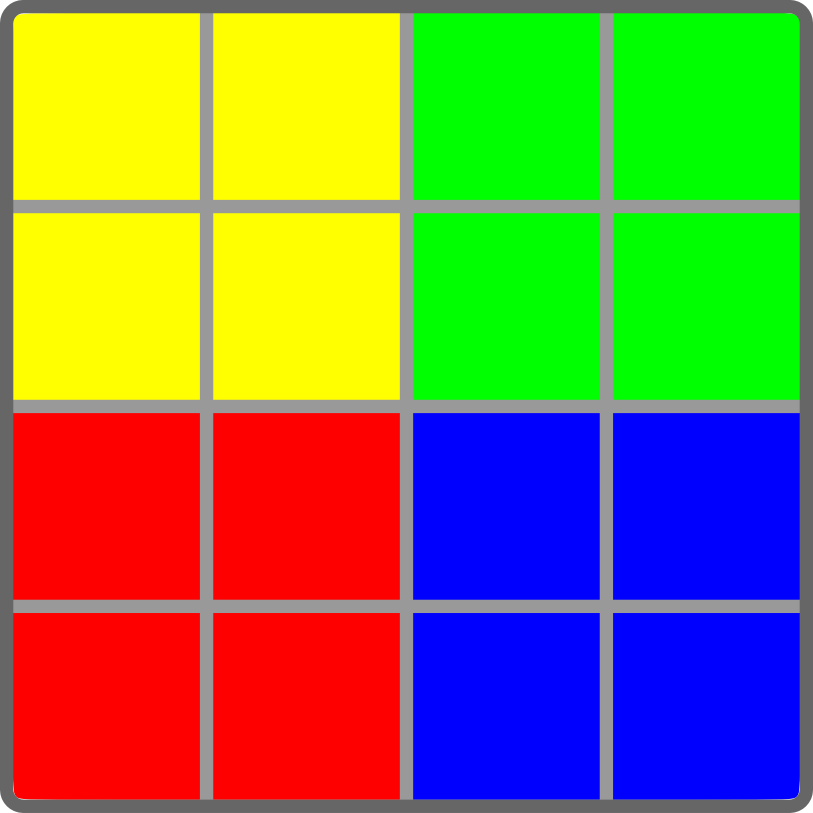
\includegraphics[width=0.55\textwidth]{images/quadraticBlockPartitioning.png}
		\caption{Quadratic block partitioning}
		\label{fig:quadraticBlockPartitioning}
	\end{subfigure}
	\caption{Row-wise, column-wise and quadratic block-wise matrix partitioning.}
	\label{fig:Partitionings}
\end{figure}

However, this approach unveils its drawbacks when multiplying two equally partitioned matrices $A$ and $B$ as illustrated in \cref{fig:rowPartitioningMM}.
In such a case, the row $r$ of $A$ and the complete matrix $B$ is needed to calculate the resulting row with index $r$.
This circumstance implies a complete repartitioning of $B$.
The repartitioning is especially grave, since $B$ has to be broadcasted to every row of $A$.

\begin{figure}[!h]
	\centering
	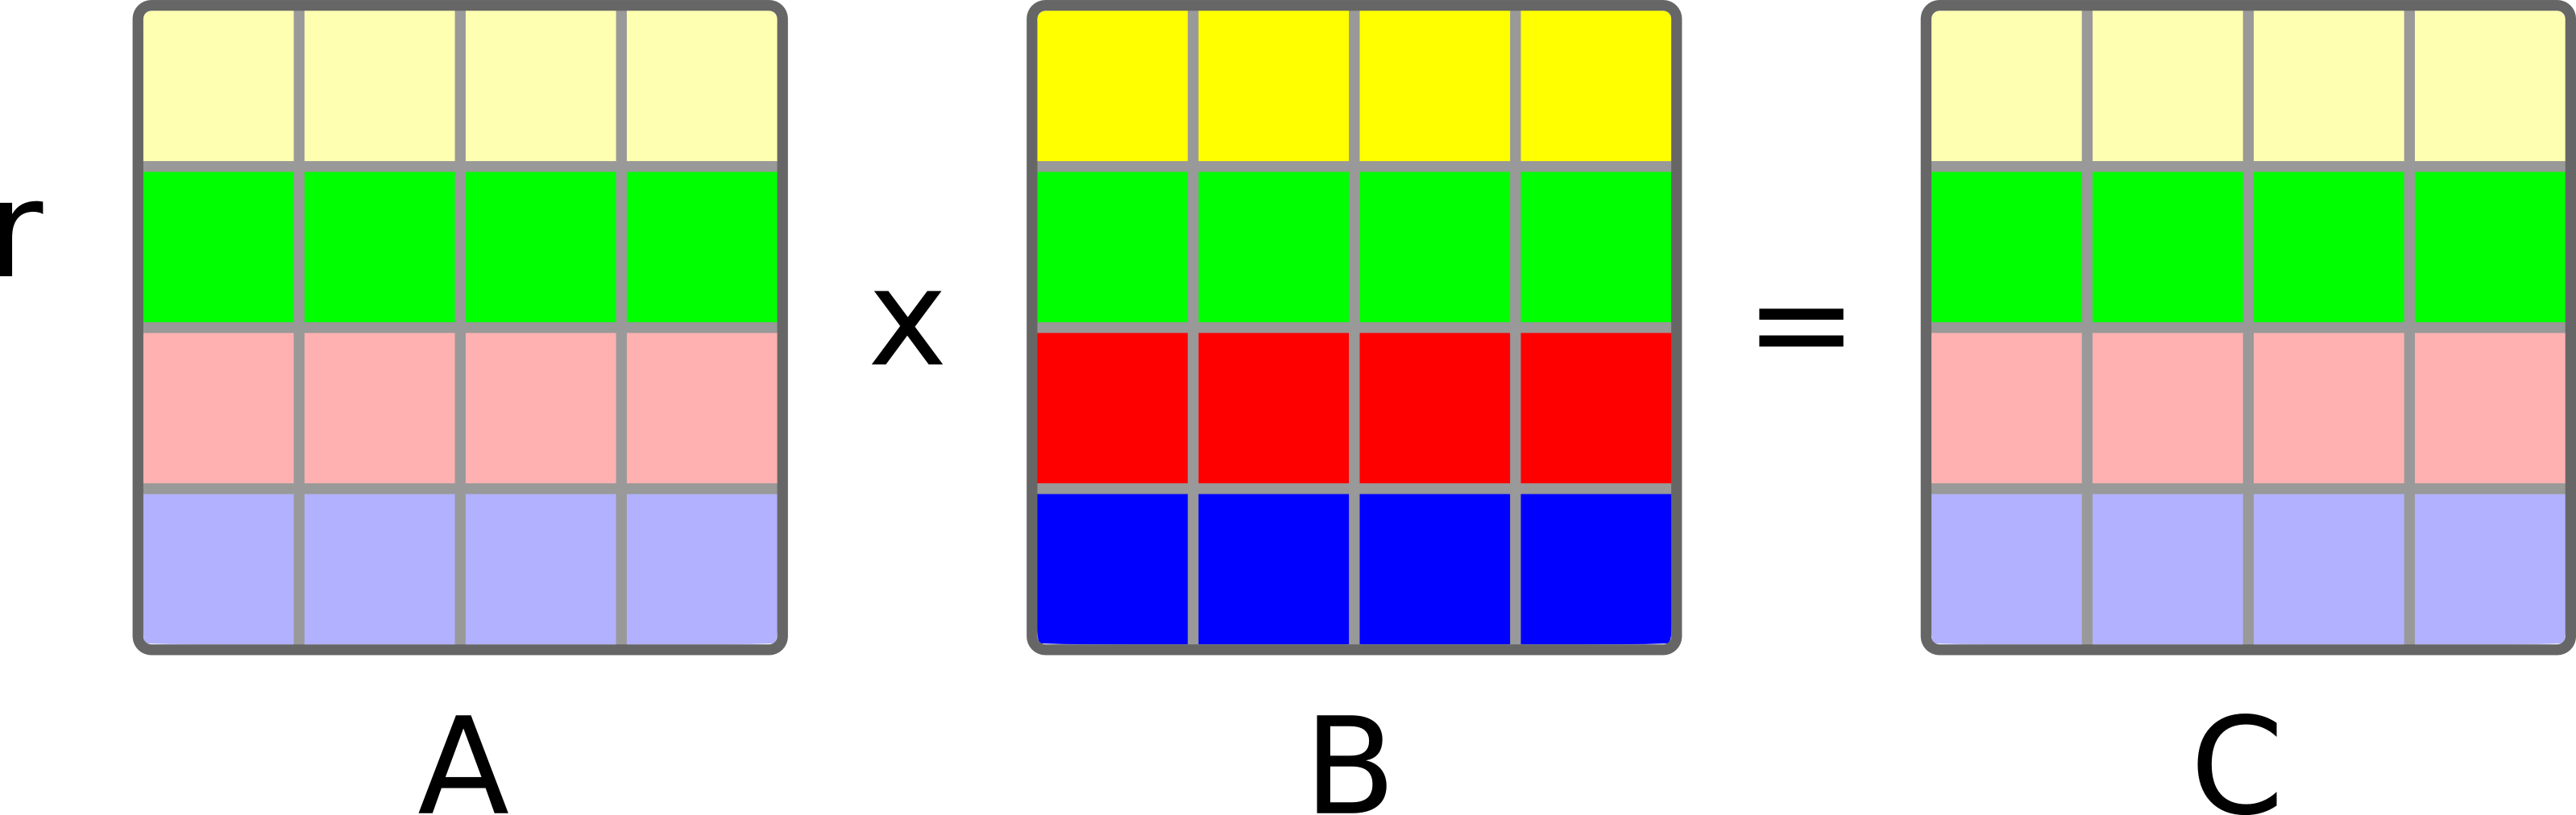
\includegraphics[width=0.6\linewidth]{images/rowMM.png}
	\caption{Matrix multiplication of $A$ and $B$. The required data to calculate row $r$ are highlighted.}
	\label{fig:rowPartitioningMM}
\end{figure}

In order to quantify the repartitioning costs of such a matrix multiplication, a simple cost model is developed.
First of all, it is limited to modeling the communication costs, since network I/O usually constitutes the bottleneck of distributed systems and is thus the dominating factor.
For the sake of simplicity, the multiplication of two quadratic matrices $A \in \mathbb{R}^{n\times n}$ and $B \in \mathbb{R}^{n\times n}$ giving the matrix $C\in \mathbb{R}^{n \times n}$ is considered.
Moreover, we assume that there are $n$ worker nodes available, each of which receiving a single row of $A$ and $B$, respectively.
Thus, $A$ and $B$ are row-wise partitioned.
We further assume that rows with the same index are kept on the same worker node.

Each row $a_r$ requires the complete knowledge of matrix $B$ in order to produce the row $c_r$.
Therefore, every row $b_r$ has to be sent to all other worker nodes.
Thus, the number of rows sent by each worker node is $n-1$.
All of the $n$ worker nodes have to do the same.
Consequently, the total number of sent messages is $n(n-1)$ and each message has a size of $n\alpha$ where $\alpha$ is the size of a matrix entry.
Usually, each sending operation causes some constant overhead inflicted by resource allocation.
Before sending the actual data over the network, memory to transfer the data to the network interface has to be allocated, network resources have to be reserved and a network connection with the remote peer has to be established.
This overhead is denoted by $\Delta$.
Since all sending operations occur in parallel, the costs caused by constant overhead are $(n-1)\Delta$.
The total amount of data, which has to sent over the network, is $n^2(n-1)\alpha$.
The network interconnection is assumed to guarantee every node a bandwidth $\nu$.
Therefore, the time needed for sending the data is $\frac{n^2(n-1)\alpha}{\nu}$.
These considerations lead to the following repartitioning cost model:

\begin{displaymath}
	cost_{row} = \frac{n^2(n-1)\alpha}{\nu} + (n-1)\Delta
\end{displaymath}

Row and column partitioning are extreme forms of blocking.
A less extreme form would be to split the matrix into equally sized quadratic blocks as shown in \cref{fig:quadraticBlockPartitioning}.
In order to identify the individual blocks, each of them will be assigned a block row and block column index assigned.
Thus, blocking adds some memory overhead in the form of index information.
An example of a $4\times 4$ matrix partitioned into $2\times 2$ blocks can be seen in \cref{fig:quadraticBlockPartitioningDetailed}.

\begin{figure}[!h]
	\centering
	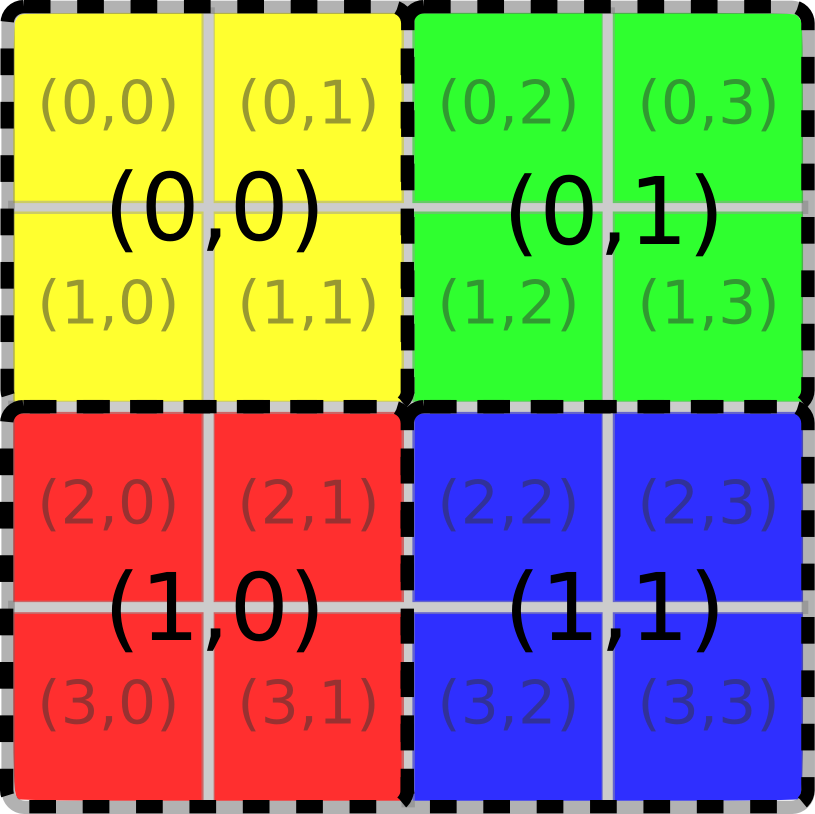
\includegraphics[width=0.25\linewidth]{images/quadraticBlockPartitioningDetailed.png}
	\caption{Detailed quadratic block partitioning with the added block row and block column indices.}
	\label{fig:quadraticBlockPartitioningDetailed}
\end{figure}

The blocks are distributed across the worker nodes.
The block size directly controls the granularity of the partitioning.
Increasing the block size will reduce the memory overhead of distributed matrices while reducing the degree of parallelism.
Thus, the user has to adjust the block size value depending on the matrix sizes and the number of available worker nodes in order to obtain best performance.

The quadratic block partitioning has similar properties like the row- and column-wise partitioning scheme when it comes to cellwise operations.
We simply have to join corresponding blocks with respect to the pair of block row and column index and execute the operation on matching blocks locally.
But how does this pattern performs for matrix multiplications?

The assumptions are the same as before and additionally it is assumed that $n$ is a square number.
Since the matrices $A$, $B$ and $C$ are equally partitioned into square blocks, indices will henceforth reference the block and not the matrix entry.
In order to calculate the block $c_{ij}$, we have to know the block row $a_{i}$ and the block column $b_{j}$.
The resulting block will be stored on the node $n_{ij}$ which already contains the blocks $a_{ij}$ and $b_{ij}$.
Thus, each node $n_{ij}$ has to receive the missing $2\left(\sqrt{n}-1\right)$ blocks from the block row $a_{i}$ and block column $b_{j}$.
In total, all worker nodes have to send $2n\left(\sqrt{n}-1\right)$ blocks.
Each block has the size $n\alpha$.
The total communication costs comprises the transmission costs and the network overhead:

\begin{displaymath}
	cost_{squareBlock} = \frac{2n^2\left(\sqrt{n}-1\right)\alpha}{\nu} + 2\left(\sqrt{n}-1\right)\Delta
\end{displaymath}

We see that the term $(n-1)$ is replaced by $2\left(\sqrt{n}-1\right)$ in the square block cost model.
For $n>2$, the square block partitioning scheme is thus superior to the row- and column-wise partitioning pattern with respect to the cost model.
The reason for this outcome is that the square blocks promote more localized computations compared to the other partitionings.
Instead of having to know the complete matrix $B$, we only have to know one block row of $A$ and one block column of $B$ to compute the final result.

Due to these advantages and also considering its simplicity, we decide to implement the square block partitioning scheme in Gilbert.
It would also be possible to combine different partitionings and select them dynamically based on the data sizes and input partitionings.

Besides the partitioning, Gilbert also has to represent the individual matrix blocks.
There exist several storing schemes for matrices depending on the sparsity of the matrix.
For example, if a matrix is dense, meaning that it does not contain many zero elements, the elements are best stored in a continuous array.
If a matrix is sparse, then a hash map or some form of compressed representation are best suited.
Gilbert chooses the representation of each block dynamically.
Depending on the non-zero elements to total elements ratio, a sparse or dense representation is selected.

\subsection{Linear Algebra Operations}
\label{sec:LinearAlgebraOperations}

The other aspect of writing distributed algorithms is to think about how the algorithms work with the locally available data and which data has to be communicated in order to compute the final result.
Stratosphere and Spark both offer a highly expressive programming API, which follows and extends the well-known MapReduce paradigm~\cite{dean:c2008a}.
Conceptually, a set of distributed data items, called \emph{DataSet} or \emph{RDD} (resilient distributed dataset) in the context of Stratosphere and Spark, respectively, forms the basis of both systems.
There are several ways to initially create a data set, such as reading from a file or distribution of a local collection.
Once a distributed data set is created, it can be modified by applying one of the transforming functions, namely \emph{map}, \emph{reduce}, \emph{join}, \emph{cross} or \emph{coGroup}.
These functions are borrowed from the world of functional programming, since they happen to be expressive enough and can serve as a utile abstraction for automatic parallelization.
Each of these transforming functions takes one or more data sets as inputs and produces a new distributed data set.
The distributed data sets are not computed directly but instead they generate a dataflow plan which is lazily executed later on.
Each node of the dataflow plan constitutes a function application and consequently a new data set.
The edges connect input data sets to output data sets and thus represent the data dependencies.

In order to understand how the different linear algebra operations are implemented, we will quickly revise the semantics of the transforming functions.
For a more detailed explanation, the reader is referred to~\cite{zaharia:2012a,alexandrov:2011a,battre:2010a}.
A distributed data set is a multiset of items.
An item can have a key value, which is retrieved by the $key$ function.
Each of the transforming functions is called with a user defined function (UDF), which specifies how each item is processed and what kind of item is emitted as the result.
In other words, it defines the program specific semantics of the transformation.

\begin{description}
	\item[map] The map operator is called with one input data set $A$ and a UDF. The UDF is called for each item $a\in A$ independently, producing one result item.

	\item[reduce] The reduce operator partitions the input data set $A$ into groups of items with the same key. 
		All items of each group are handed together to a call of the UDF.
		In other words, the UDF is called for each submultiset $A^\prime$ with $\forall a,b\in A^\prime : key(a) = key(b)$ and $\forall a \in A^\prime, b\in A \setminus A^\prime: key(a) \not = key(b)$.

	\item[join] The join operator joins two data sets $A$ and $B$ with respect to a key value.
		This means that a UDF is called for each pair $(a,b)$ with $a\in A$ and $b\in B$ with $key(a)=key(b)$.

	\item[cross]The cross operator can be understood as the Cartesian product.
		Given two data sets $A$ and $B$, cross calls the UDF for each pair $(a,b)$ with $a\in A$ and $b\in B$.
	\item[coGroup] The coGroup operator also takes 2 input data sets $A$ and $B$.
		It groups the elements of $A$ and $B$ according to their keys and joins the grouped submultisets.
		In other words, the UDF is called for each pair of multisets $(A^\prime, B^\prime)$ with $A^\prime \subseteq A \wedge B^\prime \subseteq B \wedge |keyset(A^\prime \cup B^\prime)| = 1$ and $keyset(A^\prime \cup B^\prime) \cap keyset((A \cup B) \setminus (A^\prime \cup B^\prime)) = \emptyset$.
		The function $keyset$ is the set of appearing keys in a set: $keyset(X) \coloneqq \{ key(x) \mid x \in X \}$.
\end{description}

Stratosphere as well as Spark offer a similar set of second-order functions comprising the abovementioned functions.
Consequently, we can develop the linear algebra operations in a general fashion and do not have to adhere to a specific framework.
In the following, we will outline the implementation behind the different intermediate operators with respect to the transforming functions.
We assume that the matrices are partitioned using the square block scheme.

The \code{ScalarMatrixTransformation} and \code{MatrixScalarTransformation} work on a matrix input and a scalar input.
The scalar input is a distributed data set with one item.
The scalar value is required at every matrix block to perform the \code{smOp} operation.
Thus, we use the cross function to pair the scalar value with every matrix block.
The resulting dataflow plan is shown in \cref{fig:planScalarMatrixTransformation}.

\begin{figure}[!h]
	\centering
	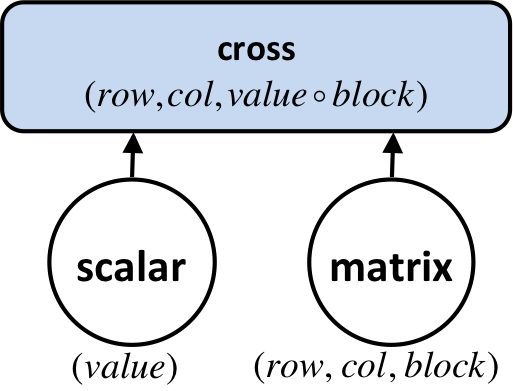
\includegraphics[width=0.25\linewidth]{images/planScalarMatrixTransformation.png}
	\caption{Dataflow plan of the \code{ScalarMatrixTransformation}.}
	\label{fig:planScalarMatrixTransformation}
\end{figure}

The \code{CellwiseMatrixTransformation} operates locally on the cells of a single matrix.
Thus, no communication is needed and the \code{unaryScalarOp} operation $f$ can be executed embarrassingly parallel.
The transformation is implemented using the map function.
The resulting dataflow plan is shown in \cref{fig:planCellwiseMatrixTransformation}.

\begin{figure}[!h]
	\centering
	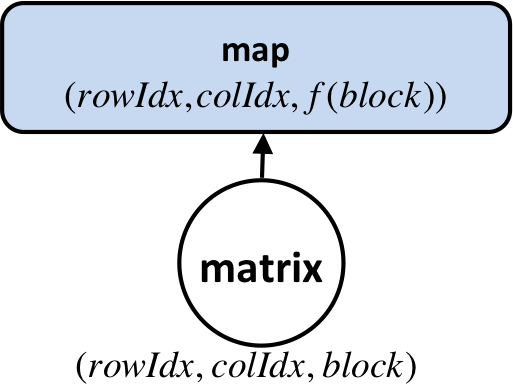
\includegraphics[width=0.25\linewidth]{images/planCellwiseMatrixTransformation.png}
	\caption{Dataflow plan of the \code{CellwiseMatrixTransformation}.}
	\label{fig:planCellwiseMatrixTransformation}
\end{figure}

The \code{CellwiseMatrixMatrixTransformation} operates locally on the cells of two matrices.
It applies an operation of type \code{scalarOp} to each pair of corresponding cell entries.
Therefore, we have to pair all matrix blocks which have the same block row and block column index.
Assuming, $f$ is the function performing the cellwise operation on the given matrix blocks, the resulting dataflow plan can be seen in \cref{fig:planCellwiseMatrixMatrixTransformation}.
The join function is represented as a join and a map node in the dataflow plan.
The map function is called for each of the matching pairs created by the join node.

\begin{figure}[!h]
	\centering
	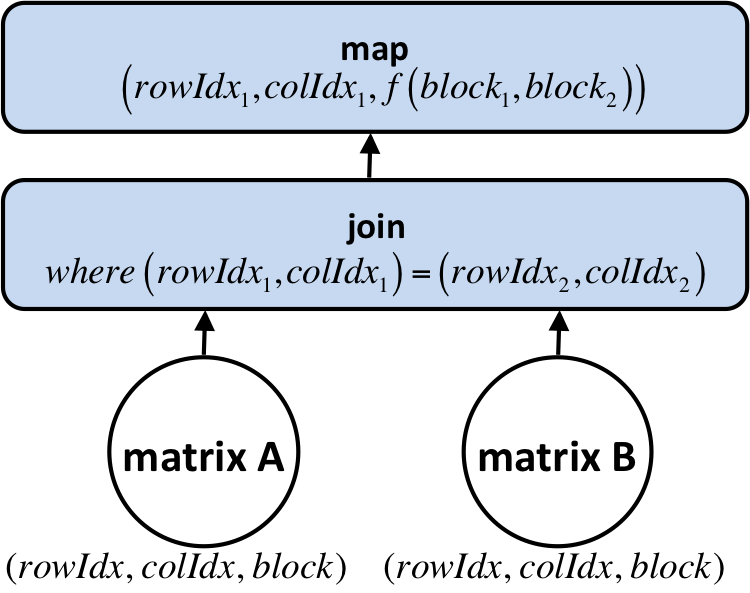
\includegraphics[width=0.365\linewidth]{images/planCellwiseMatrixMatrixTransformation.png}
	\caption{Dataflow plan of the \code{CellwiseMatrixMatrixTransformation}.}
	\label{fig:planCellwiseMatrixMatrixTransformation}
\end{figure}

Matrix multiplications are probably the most critical operation for performance in linear algebra programs.
Therefore, we have to pay attention to a thorough implementation within Gilbert.
In a MapReduce-like system there exist two distinct matrix multiplication implementations for square blocking.
The first approach is based on replicating rows and columns of the operands and is called replication based matrix multiplication (RMM).
The other method is derived from the outer product formulation of matrix multiplications.
It is called cross product based matrix multiplication (CPMM).
The RMM and CPMM methods have been implemented within SystemML~\cite{ghoting:2011a}.

Let us assume that we want to calculate $A \times B = C$ with $A,B$ and $C$ being matrices.
The block size has been chosen such that $A$ is partitioned into $m\times l$ blocks, $B$ is partitioned into $l \times n$ blocks and the result matrix $C$ will be partitioned into $m\times n$ blocks.
In order to reference the block in the $i$th block row and $j$th block column of $A$, we will write $A_{ij}$.
A block row will be denoted by a single subscript index and a block column by a single superscript index.
For example, $A_i$ marks the $i$th block row of $A$ and $A^j$ the $j$th block column of $A$.

The replication-based strategy will copy for each $C_{ij}$ the $i$th block row of $A$ and the $j$th block column of $B$.
The replicated blocks of $A_i$ and $B^j$ will be grouped together.
These steps can be achieved by a single mapper.
Once this grouping is done, the final result $C_{ij}$ can be calculated with a single reducer.
The reduce function simply has to calculate the scalar product of $A_i$ and $B^j$.
It is important to stress that $A_i$ is replicated for each $C_{ik},\forall k$.
The whole process is illustrated in \cref{fig:RMM}.

\begin{figure}[!h]
	\centering
	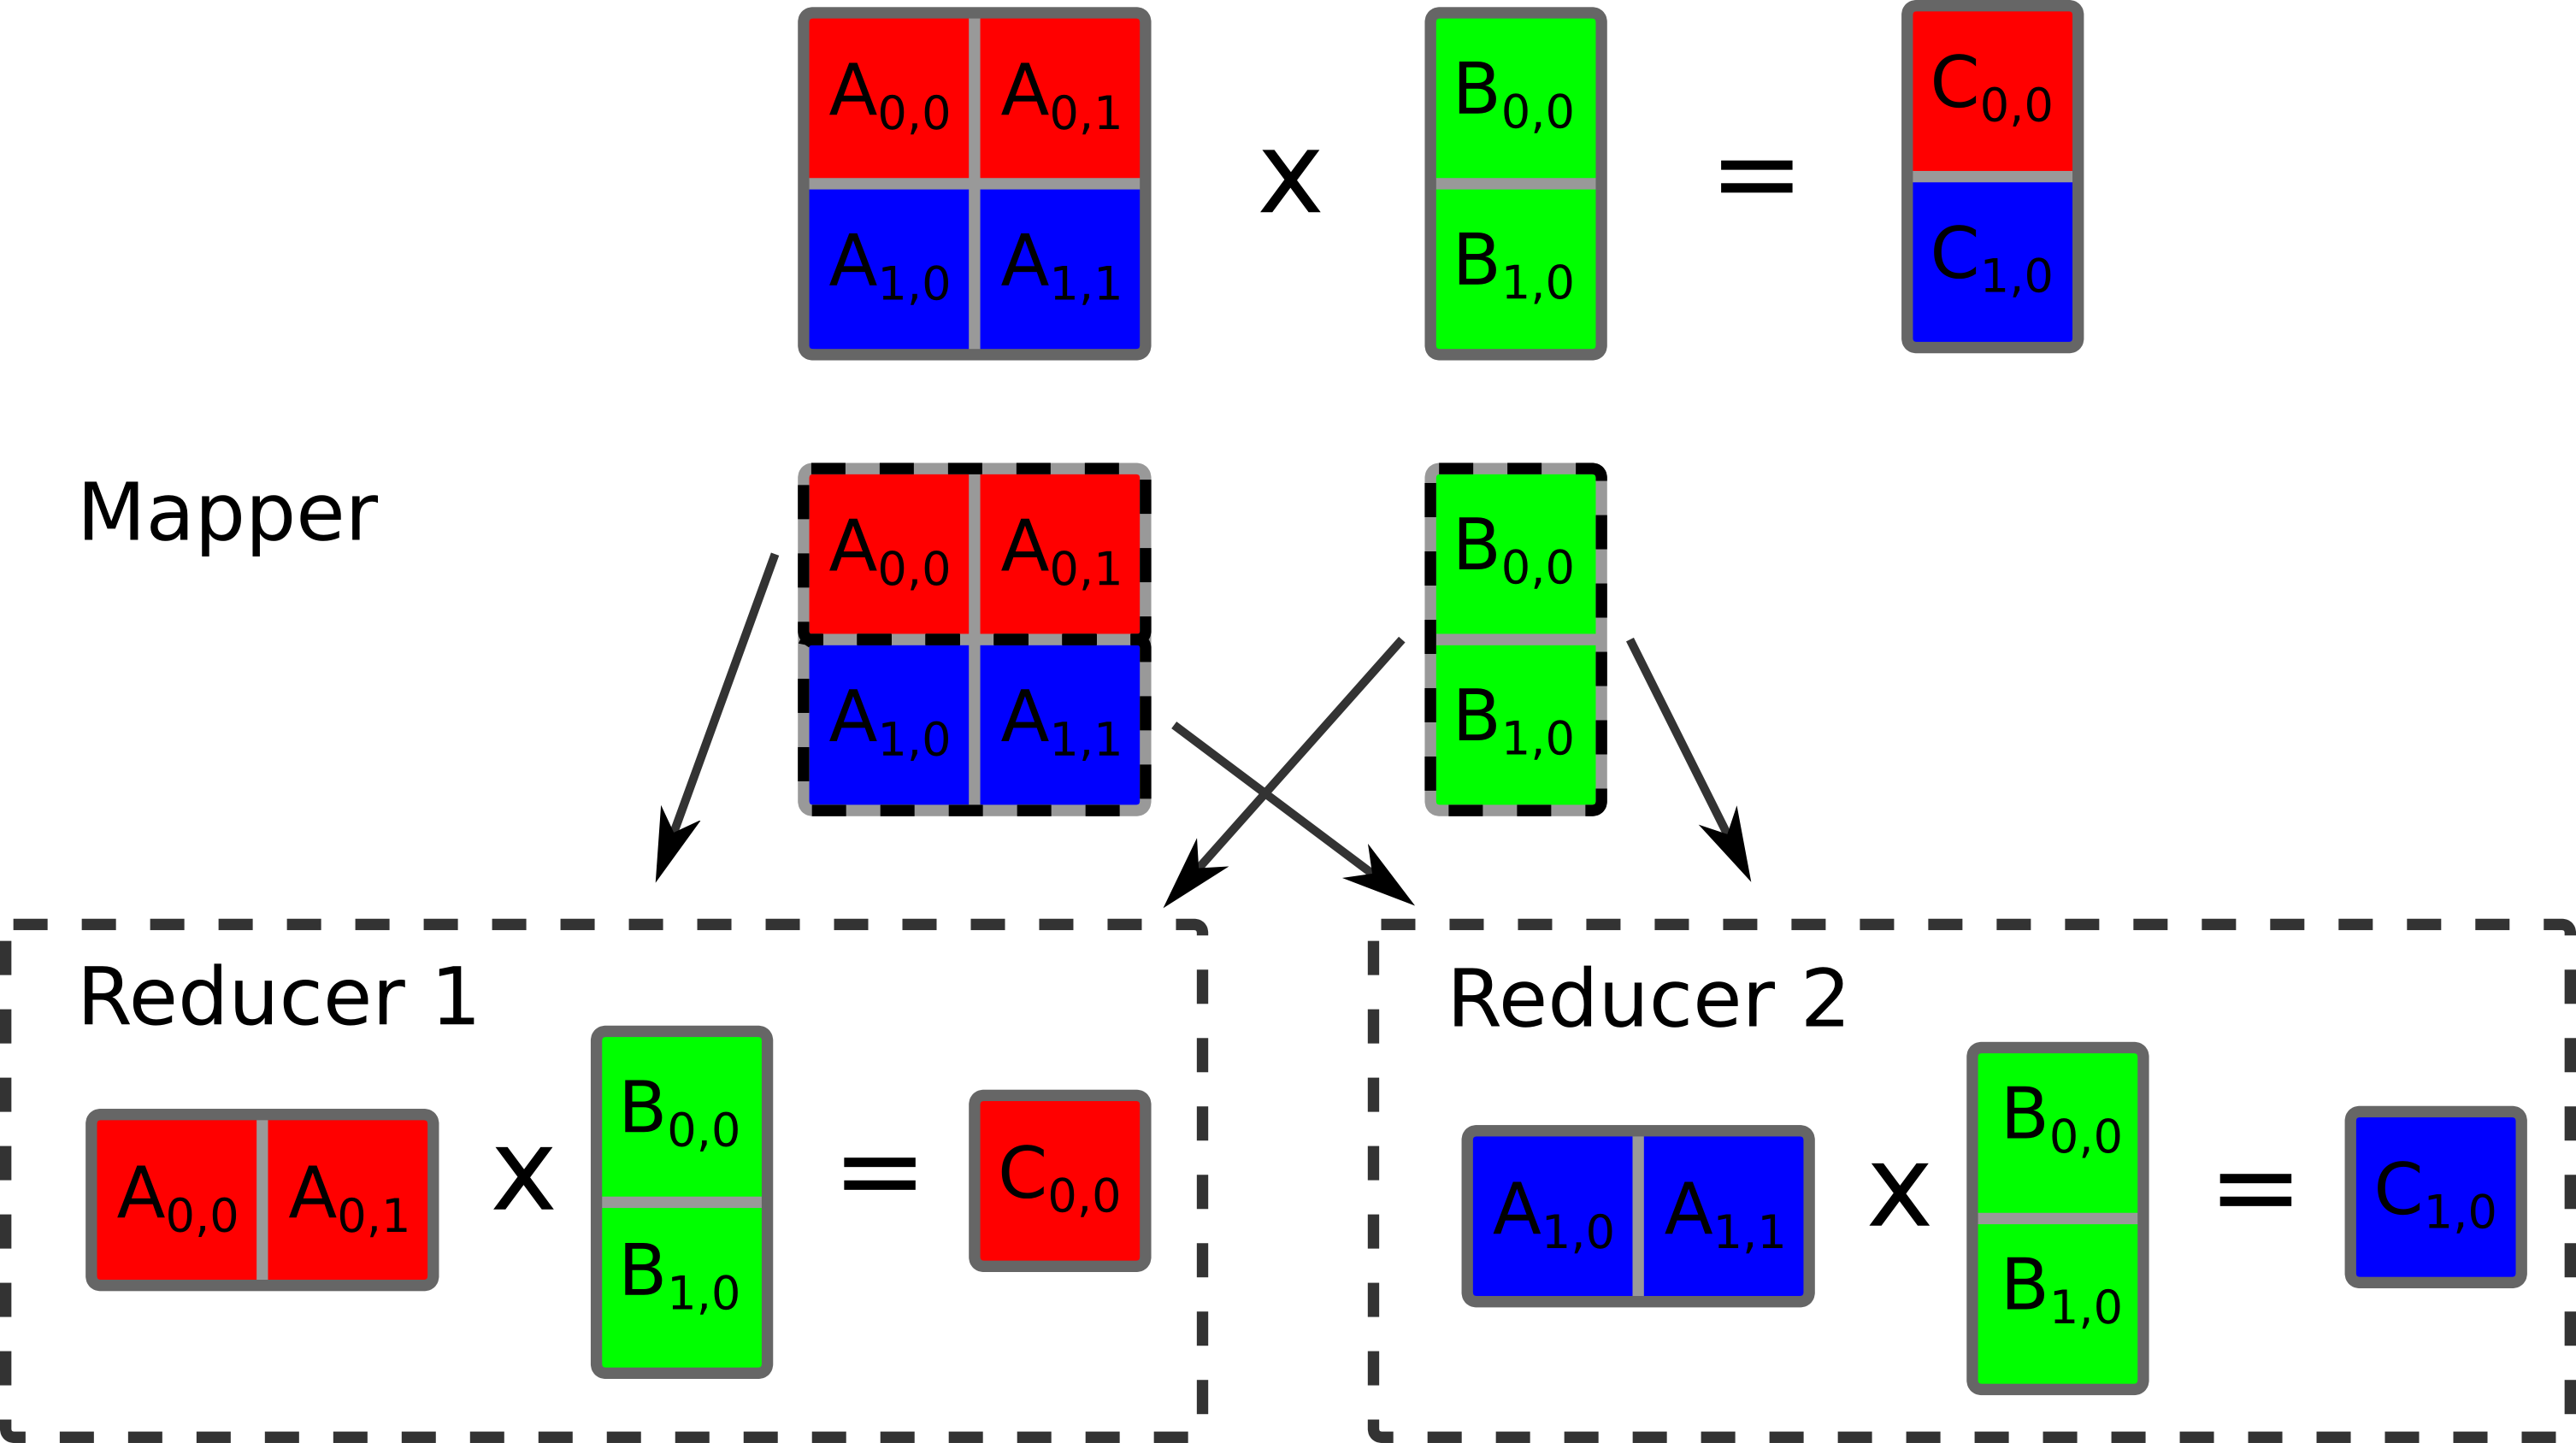
\includegraphics[width=0.4777\linewidth]{images/rmm.png}
	\caption{Replication based matrix multiplication with MapReduce.}
	\label{fig:RMM}
\end{figure}

In contrast to RMM, CPMM calculates the outer products between $A^k$ and $B_k$ for all $k$.
A mapper can group the $A^k$ and $B_k$ together so that a reducer can compute the outer products.
Consequently, this method does not replicate any data.
The outer product produces intermediate result matrices $C^k$ which have to be added up to produce the final result $C=\sum_{k=1}^{l} C^k$.
This summation can be achieved by a subsequent reducer.
The whole process is illustrated in \cref{fig:CPMM}.

\begin{figure}[!h]
	\centering
	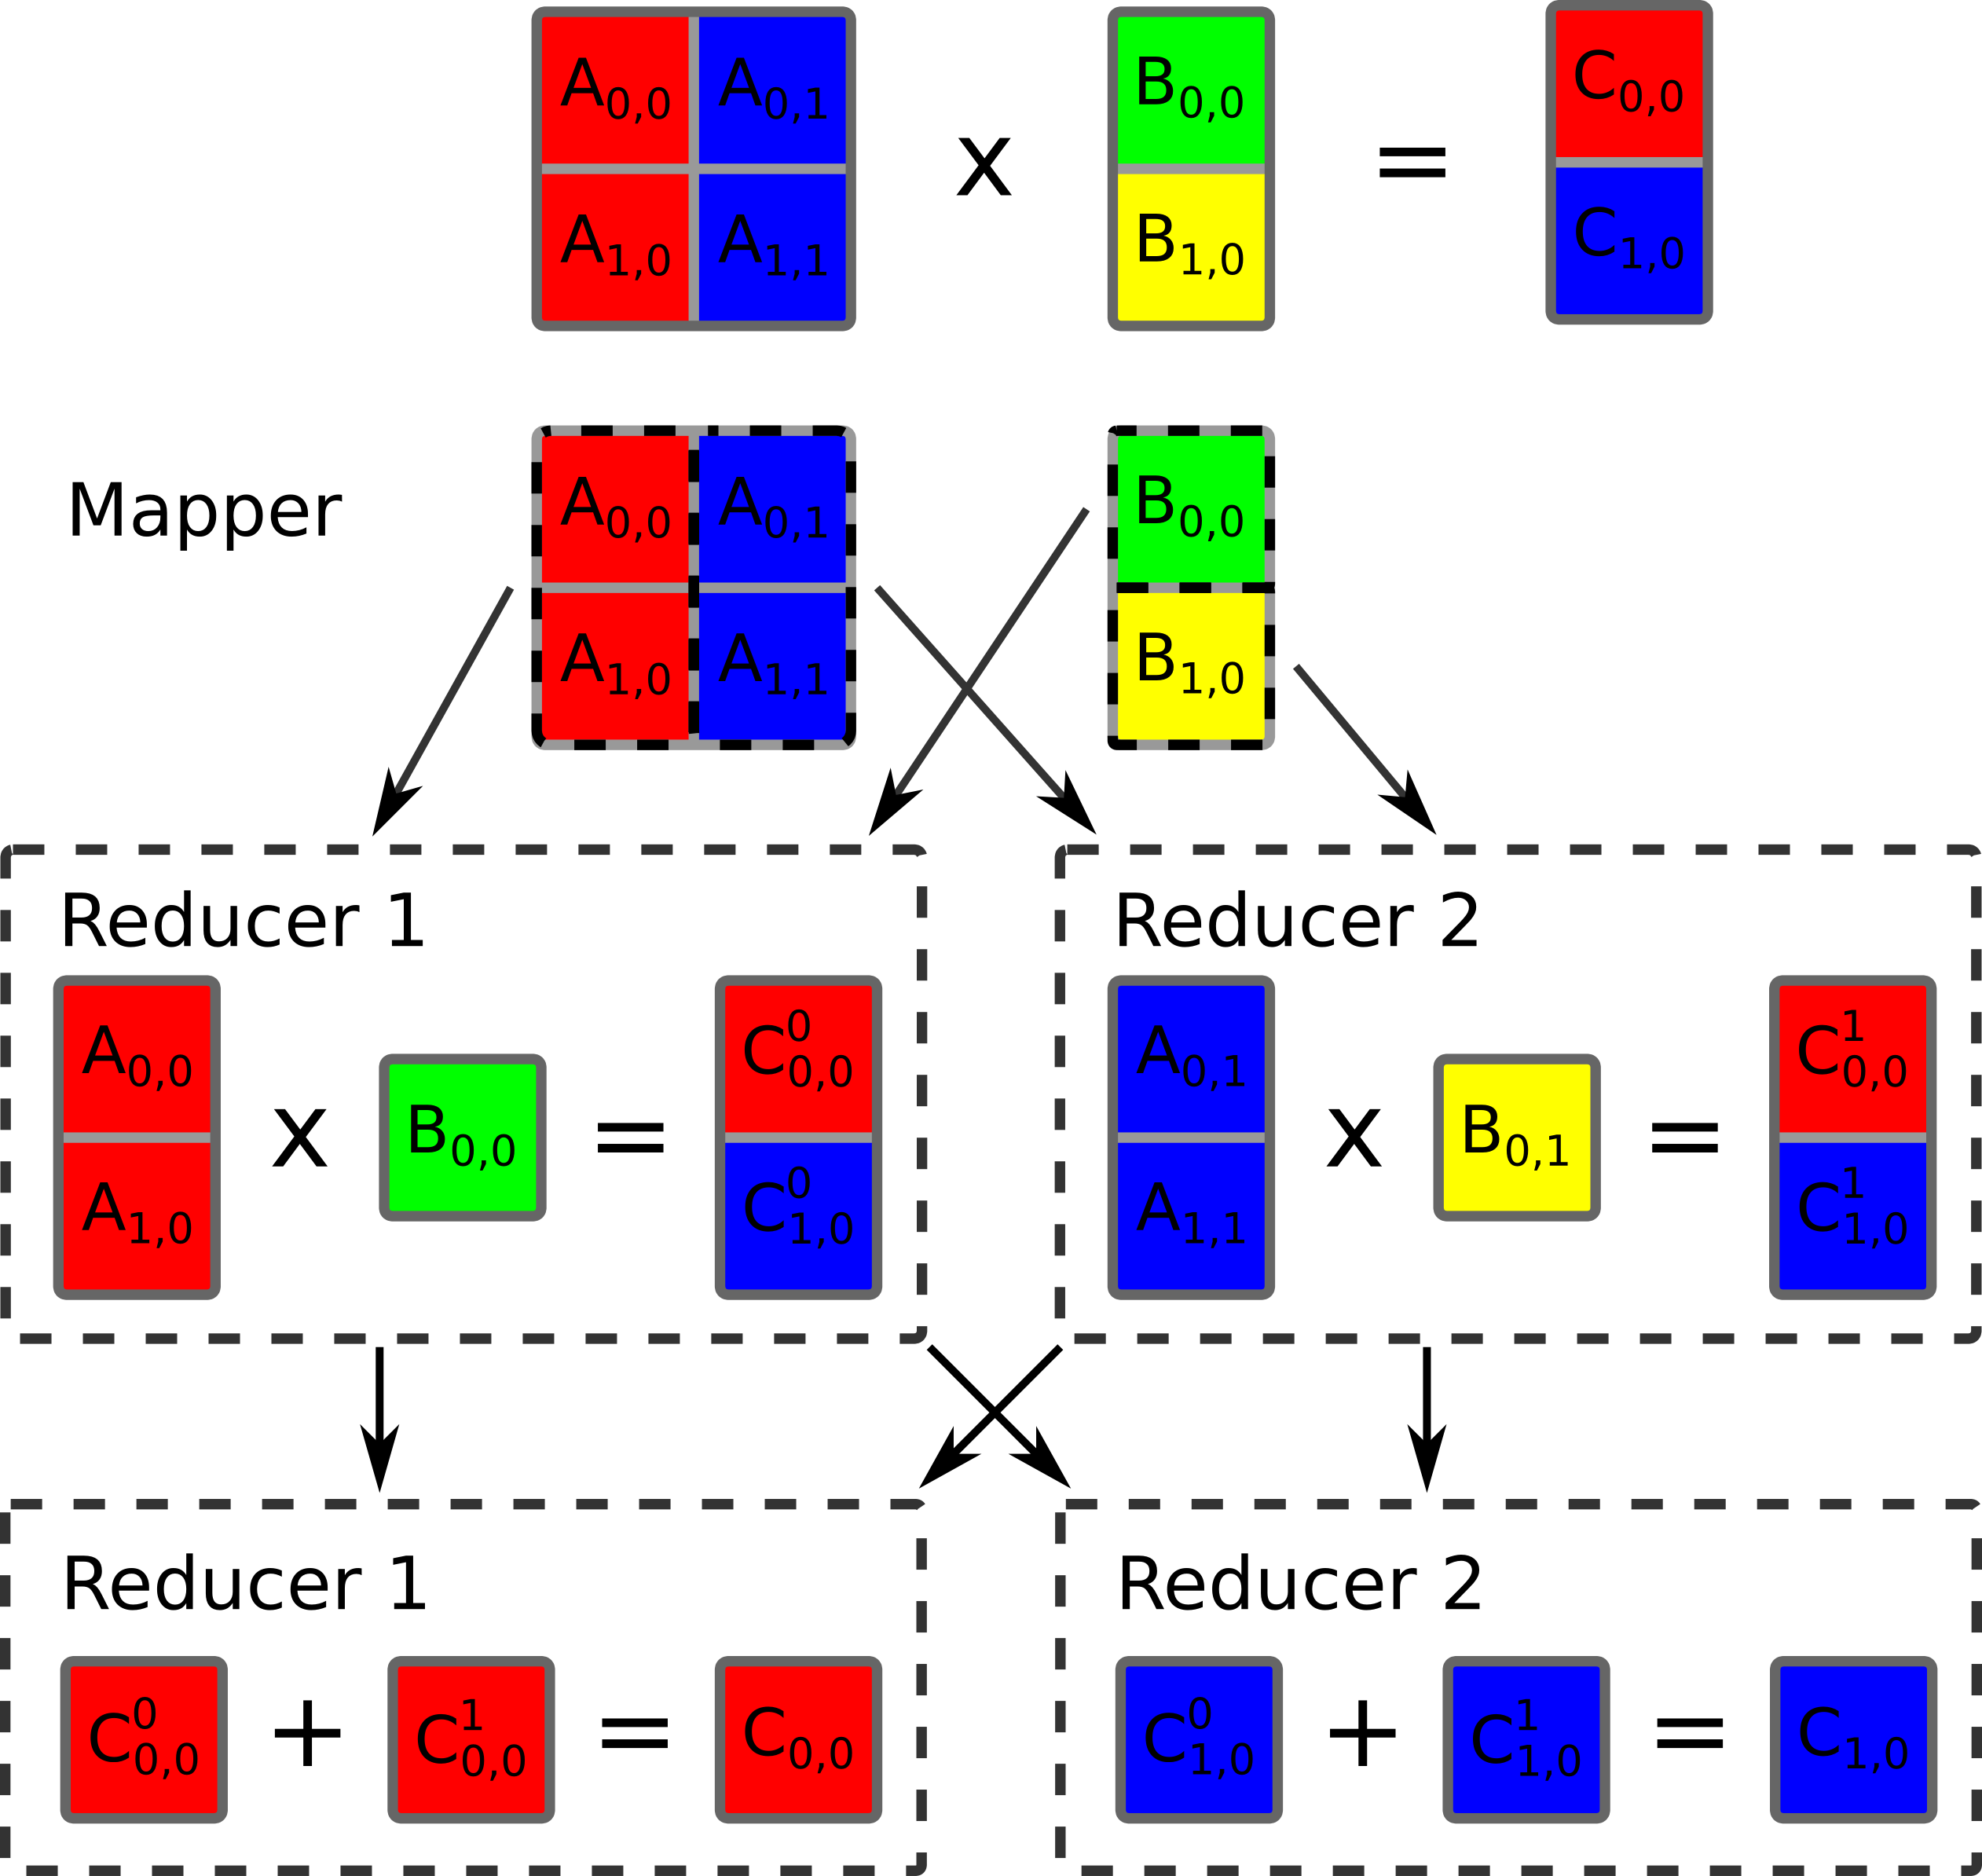
\includegraphics[width=0.4\linewidth]{images/cpmm.png}
	\caption{Cross product matrix multiplication with MapReduce.}
	\label{fig:CPMM}
\end{figure}

The methods RMM and CPMM differ in terms of network communication.
The former method can be realized within a single MapReduce job whereas the latter requires two.
Neither RMM nor CPMM is always superior.
The optimal matrix multiplication strategy depends on the matrix size of its operands $A$ and $B$.

Fortunately, Stratosphere and Spark exhibit a little bit more flexibility in terms of higher order functions.
Freed from the tight corset of the MapReduce world, matrix multiplications can be expressed more subtly.
Looking at the definition of the matrix multiplication for $C_{ij}=\sum_{k=1}^{l}A_{ik}\times B_{kj}$, it can be seen that every $A_{ik}$ has to be joined with its corresponding $B_{kj},\forall k$.
This pairwise mapping can be easily achieved by using the join function.
The join-key is the column index of $A$ and the row index of $B$.
The joiner calculates for each matching pair $A_{ik}$ and $B_{kj}$ an intermediate result $C_{ij}^k$.
Grouping the intermediate results with respect to the index pair $(i,j)$ allows us to compute the final result in a subsequent reduce step.
The overall algorithm strongly resembles the CPMM.
The corresponding dataflow plan is shown in \cref{fig:planMatrixMultiplication}.

\begin{figure}[!h]
	\centering
	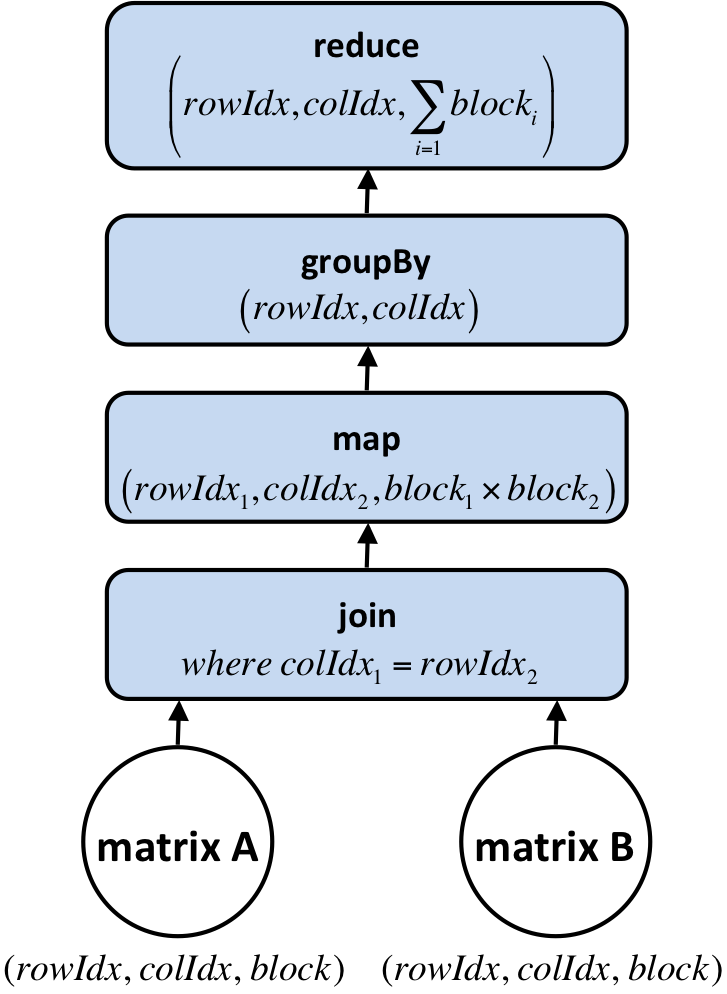
\includegraphics[width=0.354\linewidth]{images/planMatrixMultiplication.png}
	\caption{Dataflow plan of the \code{MatrixMult} operator.}
	\label{fig:planMatrixMultiplication}
\end{figure}

Stratosphere supports several execution strategies for the higher-order functions.
A cost-based optimizer selects the best strategies prior to execution.
One possible optimization concerns the join function.
The join can either be realized using a hybrid-hash join or a sort-merge join algorithm depending on the current partitioning and the input data sizes.

If one input data is relatively small compared to the other input, it is usually more efficient to use the hybrid-hash join algorithm.
Without loss of generality, we assume that the matrix $B$ constitutes such a small input.
If we further assume that the block rows of $A$ are kept on the same worker node, then the last reduce operation can be executed locally and without any shuffling.
The resulting execution plan under these assumptions is equivalent to the RMM.

If the system chooses the sort-merge join algorithm instead, then the columns of $A$ will be distributed across the worker nodes.
Consequently, the last reduce step causes a mandatory repartitioning.
Then, the resulting execution plan is equivalent to the CPMM.

Even though Gilbert has only one dataflow plan specified to implement the matrix multiplication, the Stratosphere system can choose internally between the RMM and CPMM strategy.
The strategy is selected by the optimizer which bases its decision on the data size and the partitioning, if available.
Consequently, Stratosphere frees the programmer from this decision.

The \code{VectorwiseMatrixTransformation} operator cannot be generalized independently of the \code{vectorwiseOp} operation.
For example, consider the maximum and the norm operation.
The maximum is calculated by taking the maximum of each row in a block.
Afterwards, the maximum per block is grouped with respect to the block row index and the grouped blocks are reduced by taking the maximum over all group elements.
Grouping is based on the key of each item.
The corresponding dataflow plan is shown in \cref{fig:planMaximumVectorwiseTransformation}.

\begin{figure}[!h]
	\centering
	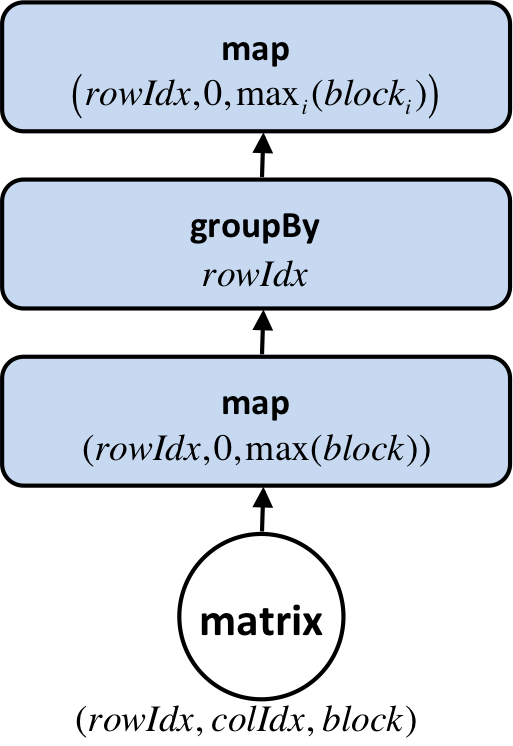
\includegraphics[width=0.25\linewidth]{images/planMaximumVectorwiseTransformation.png}
	\caption{Dataflow plan of the \code{VectorwiseMatrixTransformation} with the \code{max} operation.}
	\label{fig:planMaximumVectorwiseTransformation}
\end{figure}

In contrast to that, the $2$-norm operation requires a more sophisticated implementation.
First, the cellwise square of all matrix entries is calculated with the map function.
Then, the partial sums of every row are computed by summing the columns of each block.
This calculation constitutes another map operation.
The final row sums are calculated by grouping the partial sums with respect to their block row index and summing the items of each group up.
After this reduce operation is done, the final result is computed by taking the cellwise square root.

The \code{AggregateMatrixTransformation} operator computes an aggregate over all elements of the matrix.
Given that the aggregate operation is combinable, meaning that the aggregation can be expressed as a fold operation in terms of functional programming, we can implement it straightforwardly.
We only need a reducer with the aggregation function $f$ as UDF.
The respective dataflow plan can be found in \cref{fig:planAggregateMatrixTransformation}.
The $default$ variable holds the initial value for the fold operation.
In case that the aggregate is not combinable, it has to be implemented individually.

\begin{figure}[!h]
	\centering
	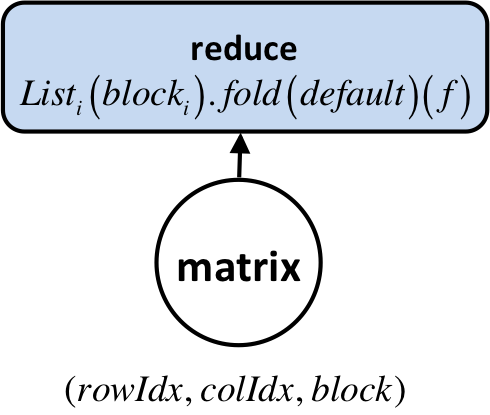
\includegraphics[width=0.25\linewidth]{images/planAggregateMatrixTransformation.png}
	\caption{Dataflow plan of the \code{AggregateMatrixTransformation}.}
	\label{fig:planAggregateMatrixTransformation}
\end{figure}

\section{Implementation}
\label{cha:implementation}

The development of Gilbert involved the implementation of the complete technology stack of a programming language.
For each technology, we had to decide how to implement it.
The lexer and parser, for example, can be automatically generated using tools such as ANTLR~\cite{antlr}, Bison~\cite{bison} or Yacc~\cite{yacc}.
However, using these tools would have required to manage the complexity of several frameworks and probably a lot of boilerplate code to fuse them together.
Therefore, we looked for a tool with the potential to implement the complete stack of Gilbert.

Fortunately, the Scala language~\cite{scala,odersky:2010a} unifies all required technologies under one umbrella.
Scala is a highly scalable language, well suited for script sized programs as well as enterprise applications.
The language combines object oriented and functional programming, giving a maximum of flexibility to the programmer.
The Scala code is compiled to Java bytecode and thus executed on a JVM.
This feature makes the language platform independent to the greatest possible extent.
Furthermore, it can integrate existing Java code and thus benefit from the rich set of Java libraries.
Last but not least, it is like the new cool kid on the block of programming languages, which everyone likes.

An important aspect of our choice was how easily a parser and a compiler can be implemented with Scala.
If one decides to implement these programs within a popular language such as Java, C/C++ or C\# and without any additional tools, then it quickly becomes a tedious and error-prone task.
That's the reason why tools like Yacc and ANTLR have emerged.
Scala circumvents this problem by providing an internal domain specific language (DSL) for an easy and quick development of parsers and lexers.
This DSL is also known as Scala Parser Combinators.
Once an abstract syntax tree has been generated using these parser combinators, it is very easy to develop a compiler using Scala's pattern matching functionality.
The pattern matching capabilities of Scala are similar to functional languages, such as Haskell, ML or OCaml.
It can even be applied on object hierarchies, making it a powerful tool for OOP and functional programming likewise.
The Scala Parser Combinators generate recursive descent parsers which are capable of parsing LL(*) grammars.

We decide to develop Gilbert as an open source project so that everyone can benefit from the project.
The complete source code is hosted on Github and is publicly accessible under \url{https://github.com/gilbert-lang/gilbert}.

\subsection{Math-Backend}
\label{sec:mathBackend}

In \cref{cha:gilbertruntime} we have explained the representation of distributed matrices and how the intermediate operators are mapped to dataflow plans.
What was left out, though, is how the local operations on the block-level are implemented.
Consider, for example, the matrix multiplication of two distributed matrices.
The result is obtained by joining the blocks of both operands, performing a local matrix multiplication on a matching block pair and reducing the intermediate results.
The local matrix multiplication is self-contained and has to be executed by some algorithm.
Since there already exist highly optimized algorithms for different matrix representations, dense or sparse, we do not have to reinvent the wheel.

One of the numerous linear algebra libraries for the Java ecosystem is Mahout~\cite{mahout:2011a}.
The math library of Mahout is mainly written in Java and thus offers a Java binding.
Initially, Mahout was used to implement the local linear algebra operations of Gilbert.
However, it quickly turned out that Mahout lacked reliable support for sparse matrices and suffered from poor performance.
Since Gilbert is geared towards being a linear algebra environment for sparse matrices with descent performance, we were forced to look for alternatives.
Next we came across Breeze~\cite{breeze}, a library for numerical processing written in Scala.

Breeze offers data structures for all linear algebra primitives, such as matrices and vectors.
Additionally, it supports sparse and dense variants.
For each version, Breeze is shipped with elaborate algorithms implementing the linear algebra operations.
In case that the host has a BLAS or LAPACK library installed, which is compiled and optimized for the underlying architecture, Breeze automatically detects and uses it.
That way, Breeze can achieve near optimal performance when multiplying dense matrices compared to compiled languages such as C/C++ and Fortran.
Under the hood, Breeze relies on the netlib-java library for this feature.
The fact that it offers a Scala binding allowed it to be integrated seamlessly into Gilbert.
We have chosen this library as our principal math back end because it is clean, very reliable and extremely powerful.

Additionally, Gilbert also supports the aforementioned Mahout library as a secondary math back end.
The user can select on demand which system he wants to use depending on his personal preference.
The inclusion of Mahout also emphasizes the extensible architecture of Gilbert.
It is very easy to add further math libraries to Gilbert.

\subsection{Execution Engines}

From the very first moment, Gilbert was intended as a general purpose linear algebra front end for different runtime systems.
Therefore, Gilbert includes an abstraction, called execution engine, which encapsulates the logic for running a Gilbert program.
Currently, Gilbert comes with three different execution engines.
The local executor serves as a reference implementation of the linear algebra operations and can be used for computing little data on a single machine.
But the purpose of Gilbert was to enable linear algebra programs to handle big data and thus a distributed execution is strictly necessary.
The Stratosphere and Spark executor fulfill that condition.
However, Gilbert is not restricted to these systems as backends.
In fact, it should be easy to add new execution engines to Gilbert.
They only have to be able to map the intermediate operators to their runtime specific implementations.
For example, an executor using a message passing system for the parallel execution is easily conceivable.
We refrained from doing it, though, because of its error-prone implementation.
We will describe the Stratosphere and Spark parallel executors and the problems we encountered while implementing Gilbert in the following subsections.

\subsubsection{Stratosphere}

The Stratosphere project is still in an early stage and thus it was not expected that the development would proceed completely smoothly.
The individual intermediate operators are implemented as described in \cref{sec:LinearAlgebraOperations}.
However, the iteration mechanism of Stratosphere was slightly flawed.
It was not possible to reuse expressions which were used outside of the loop.
The system would generate a completely new instance of the expression in that case.
This behavior not only degraded the overall performance but also corrupted the consistency of Gilbert programs.
A random matrix, for example, would have had two different values: One outside of the loop and another one inside of the loop.
Therefore, we had to fix this problem within Stratosphere to guarantee a correct functioning of Gilbert.

Another problem was that Stratosphere did not support the transmission of implicit values such as a context bound.
These would have been necessary to implement a generic matrix being parameterized on the type of its elements.
The Breeze library would have required the additional information for a proper functioning.
Therefore, we had to instantiate a concrete matrix implementation for each element type we needed.
This clumsy solution leads to code duplication at some points.

\subsubsection{Spark}

The development of the Spark executor was comparable to the Stratosphere executor.
The intermediate operators could be implemented almost identically.
Furthermore, we could reuse the distributed matrices defined for Stratosphere and the math back end.
In conclusion, the development process proceeded without major problems. 